\documentclass[a4paper]{article}

\usepackage[T1]{fontenc}
\usepackage[utf8]{inputenc}
\usepackage{mlmodern}

%\usepackage{ngerman}	% Sprachanpassung Deutsch

\usepackage{graphicx}
\usepackage{geometry}
\geometry{a4paper, top=15mm}

\usepackage{subcaption}
\usepackage[shortlabels]{enumitem}
\usepackage{amssymb}
\usepackage{amsthm}
\usepackage{amsmath}
\usepackage{mathtools}
\usepackage{braket}
\usepackage{bbm}
\usepackage{graphicx}
\usepackage{float}
\usepackage{yhmath}
\usepackage{tikz}
\usepackage{scratch}
\usetikzlibrary{patterns,decorations.pathmorphing,positioning}
\usetikzlibrary{calc,decorations.markings}

\usepackage[backend=biber, sorting=none]{biblatex}
\addbibresource{cite.bib}

\usepackage[framemethod=TikZ]{mdframed}

\tikzstyle{titlered} =
    [draw=black, thick, fill=white,%
        text=black, rectangle,
        right, minimum height=.7cm]


\usepackage[colorlinks=true,naturalnames=true,plainpages=false,pdfpagelabels=true]{hyperref}
\usepackage[parfill]{parskip}
\usepackage{lipsum}

\usepackage{tcolorbox}
\tcbuselibrary{skins,breakable}

\pagestyle{myheadings}

\colorlet{colexam}{black}
\newcounter{definition}
\newtcolorbox[use counter=definition]{mydef}[1]{
    empty,
    title={\textbf{Definition~\thetcbcounter}~~(\textit{#1})},
    attach boxed title to top left,
    fontupper=\sl,
    boxed title style={
        empty,
        size=minimal,
        bottomrule=1pt,
        top=1pt,
        left skip=0cm,
        overlay=
            {\draw[colexam,line width=1pt]([yshift=-0.4cm]frame.north
        west)--([yshift=-0.4cm]frame.north east);}},
            coltitle=colexam,
            fonttitle=\normalfont,
            before=\par\medskip\noindent,
            parbox=false,
            boxsep=-1pt,
            left=0.75cm,
            right=3mm,
            top=4pt,
            breakable,
            pad at break*=0mm,
            vfill before first,
            overlay unbroken={
                \draw[colexam,line width=1pt]
                ([xshift=0.6cm, yshift=-0.5pt]frame.south
                west)--([xshift=0.6cm,yshift=-1pt]frame.north west)
                --([xshift=0.6cm]frame.south west)--([xshift=-13cm]frame.south east); },
            overlay first={
                \draw[colexam,line width=1pt]
                ([xshift=0.6cm, yshift=-0.5pt]frame.south
                west)--([xshift=0.6cm,yshift=-1pt]frame.north west)
                --([xshift=0.6cm]frame.south west); },
            overlay last={
                \draw[colexam,line width=1pt]
                ([xshift=0.6cm, yshift=-0.5pt]frame.south
                west)--([xshift=0.6cm,yshift=-1pt]frame.north west)
                --([xshift=0.6cm]frame.south west)--([xshift=-13cm]frame.south east); }
}
\newcounter{theorem}
\newtcolorbox[use counter=theorem]{theorem}{
    empty,
    title={Theorem ~\thetcbcounter},
    attach boxed title to top left,
    fontupper=\sl,
    boxed title style={
        empty,
        size=minimal,
        bottomrule=1pt,
        top=1pt,
        left skip=0cm,
        overlay=
            {\draw[colexam,line width=1pt]([yshift=-0.4cm]frame.north
        west)--([yshift=-0.4cm]frame.north east);}},
            coltitle=colexam,
            fonttitle=\bfseries,
            before=\par\medskip\noindent,
            parbox=false,
            boxsep=-1pt,
            left=0.75cm,
            right=3mm,
            top=4pt,
            breakable,
            pad at break*=0mm,
            vfill before first,
            overlay unbroken={
                \draw[colexam,line width=1pt]
                ([xshift=0.6cm, yshift=-0.5pt]frame.south
                west)--([xshift=0.6cm,yshift=-1pt]frame.north west)
                --([xshift=0.6cm]frame.south west)--([xshift=-13cm]frame.south east); },
            overlay first={
                \draw[colexam,line width=1pt]
                ([xshift=0.6cm, yshift=-0.5pt]frame.south
                west)--([xshift=0.6cm,yshift=-1pt]frame.north west)
                --([xshift=0.6cm]frame.south west); },
            overlay last={
                \draw[colexam,line width=1pt]
                ([xshift=0.6cm, yshift=-0.5pt]frame.south
                west)--([xshift=0.6cm,yshift=-1pt]frame.north west)
                --([xshift=0.6cm]frame.south west)--([xshift=-13cm]frame.south east); }
}
\newcounter{lemma}
\newtcolorbox[use counter=lemma]{lemma}{
    empty,
    title={Lemma~\thetcbcounter},
    attach boxed title to top left,
    fontupper=\sl,
    boxed title style={
        empty,
        size=minimal,
        bottomrule=1pt,
        top=1pt,
        left skip=0cm,
        overlay=
            {\draw[colexam,line width=1pt]([yshift=-0.4cm]frame.north
        west)--([yshift=-0.4cm]frame.north east);}},
            coltitle=colexam,
            fonttitle=\bfseries,
            before=\par\medskip\noindent,
            parbox=false,
            boxsep=-1pt,
            left=0.75cm,
            right=3mm,
            top=4pt,
            breakable,
            pad at break*=0mm,
            vfill before first,
            overlay unbroken={
                \draw[colexam,line width=1pt]
                ([xshift=0.6cm, yshift=-0.5pt]frame.south
                west)--([xshift=0.6cm,yshift=-1pt]frame.north west)
                --([xshift=0.6cm]frame.south west)--([xshift=-13cm]frame.south east); },
            overlay first={
                \draw[colexam,line width=1pt]
                ([xshift=0.6cm, yshift=-0.5pt]frame.south
                west)--([xshift=0.6cm,yshift=-1pt]frame.north west)
                --([xshift=0.6cm]frame.south west); },
            overlay last={
                \draw[colexam,line width=1pt]
                ([xshift=0.6cm, yshift=-0.5pt]frame.south
                west)--([xshift=0.6cm,yshift=-1pt]frame.north west)
                --([xshift=0.6cm]frame.south west)--([xshift=-13cm]frame.south east); }
}

\newcommand{\eps}{\varepsilon}
\usepackage[OT2,T1]{fontenc}
\DeclareSymbolFont{cyrletters}{OT2}{wncyr}{m}{n}
\DeclareMathSymbol{\Sha}{\mathalpha}{cyrletters}{"58}

\markright{Popović\hfill Seminar\hfill}


\title{University of Vienna\\
\vspace{1cm}Seminar:\\Joint RICAM Seminar\\
\vspace{0.5cm}
Summary of talk by Otmar Scherzer
}
\author{Milutin Popovic}


\begin{document}

\maketitle
\tableofcontents

\section{Governing Equations of Fluid Dynamics}
We first of start with a fluid with density/mass
\begin{align}
    \rho(\mathbf{x}, t),
\end{align}
with a position $\mathbf{x} = (x, y, z)$ in three dimensional space at time
$t$. For water-wave applications, we should note that we take
$\rho=\text{constant}$. The fluid moves in time and space with a velocity field
\begin{align}
    \mathbf{u}(\mathbf{x}, t) = (u, v, w).
\end{align}
Additionally it is also described by the pressure of the fluid
\begin{align}
    P(\mathbf{x}, t),
\end{align}
generally depending on time and position. When thinking of e.g. water the
pressure increases the deeper we go, that is with decreasing or increasing $z$
coordinate (depending how we set up our system $z$ pointing up or down
respectively).

The general assumption in fluid dynamics is the \textbf{Continuum
Hypothesis}, which assumes continuity of $\textbf{u}, \rho$ and $P$ in
$\mathbf{x}$ and $t$. In other words, we premise that the velocity field,
density and pressure are ''nice enough`` functions of position and time, such
that we can do all the differential operations we desire in the framework of
fluid dynamics.
\subsection{Mass Conservation}
Our aim is to derive a model of the fluid and its dynamics, with respect to
time and position, in the most general way. This is generally done thinking
of the density of a given fluid, which is a unit of mass per unit volume,
intrinsically  an integral representation to derive these equations is going
to be used.

Let us now thing of an arbitrary fluid. Within this fluid we define a fixed
volume $V$ relative to a chosen inertial frame and bounded by a surface $S$
within the fluid, such that the fluid motion $\mathbf{u}(\mathbf{x}, t)$ may
cross the surface $S$. The fluid density is given by $\rho(\mathbf{x}, t)$,
thereby the mass of the fluid in the defined Volume $V$ is an integral
expression
\begin{align}
    m = \int_V \rho(\mathbf{x}, t) dV.
\end{align}
The figure bellow \ref{fig:volume}, expresses the above described picture.
\begin{figure}[H]
    \centering
  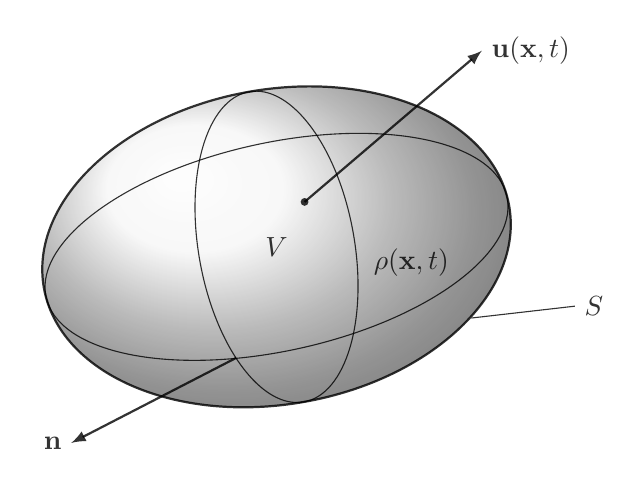
\begin{tikzpicture}[>=latex,scale=1, xscale=1, opacity=.8]
% second sphere
    \begin{scope}[rotate=10, xscale=3, yscale=2, shift={(2.3,-0.2)}]
      \coordinate (O) at (0,0);
      \shade[ball color=gray!10!] (0,0) coordinate(Hp) circle (1) ;

      \draw[thick] (O) circle (1);
      \draw[rotate=5] (O) ellipse (1cm and 0.66cm);
      \draw[rotate=90] (O) ellipse (1cm and 0.33cm);
\node[circle, fill=black, inner sep=1pt] at (0.15, 0.25) {} ; \draw[-latex, thick] (0.15, 0.25) -- (1, 1) ;
      \node[right] at (1, 1) {$\mathbf{u}(\mathbf{x}, t)$};

      \node[] at (O) {$V$};
      \node[] at (0.55, -0.25) {$\rho(\mathbf{x}, t)$};

      \draw[-] (0.76, -0.66) -- (1.2, -0.7);
      \node[right] at (1.2, -0.7) {$S$};

      \draw[-latex, thick] (-0.25, -0.65) -- (-1, -1);
      \node[left] at (-1, -1) {$\mathbf{n}$};

    \end{scope}

% axis
  \end{tikzpicture}
  \caption{Volume bounded by a surface in a fluid with density and momentum,
  with a surface normal vector $\mathbf{n}$ \label{fig:volume}}
\end{figure}

Since we want to figure out the fluid dynamics, we can consider now the rate
of change of mass in of this completely arbitrary $V$, which needs to be
disappear, i.e. is equal to zero since we cannot lose mass. Matter (mass) is
neither created nor destroyed anywhere in the fluid
\begin{align}
    \frac{d}{dt}\left( \int_V \rho(\mathbf{x}, t)\ dV \right) = 0.
\end{align}
We may get more information with simply ''differentiating under the integral
sign``, also known as the Leibniz Rule of Integration, see appendix
\ref{appendix:leibniz}, the above integral equation reads
\begin{align}\label{eq:mass balance}
    \frac{dm}{dt} = \int_V \frac{\partial \rho(\mathbf{x}, t)}{\partial t}\ dV
    +\int_{\partial V} \rho(\mathbf{x}, t) \mathbf{u}\cdot\mathbf{n}\ dS
    = 0.
\end{align}
The above equation \ref{eq:mass balance} is an underlying equation, describing that the rate of
change of mass in V is brought about, only by the rate of mass flowing into
V across S, and thus the mass does not change.

For the second integral in \ref{eq:mass balance} we utilize the Gaussian
integration law to acquire an integral over the volume
\begin{align}
    \int_{\partial V} \rho(\mathbf{x}, t) \mathbf{u} \cdot \mathbf{n} \ dS =
    \int_V \nabla (\rho \mathbf{u})\ dV.
\end{align}
Thereby we can put everything inside the volume integral
\begin{align}
    \frac{d m}{dt} = \int_V \left(\partial_t \rho + \nabla(\rho \mathbf{u}) \right) \ dV = 0.
\end{align}
Everything under the integral sign needs to be zero, thus we obtain
the \textbf{Equation of Mass Conservation} or in the general sense also
called the \textbf{Continuity Equation}
\begin{align}\label{eq:continuity}
    \partial_t \rho + \nabla(\rho \mathbf{u}) = 0
\end{align}

In the light of the results of the equation of mass conservation
\ref{eq:continuity}, an expansion, of the nabla gives
\begin{align}
    \partial_t \rho + (\nabla \rho)\mathbf{u} + \rho(\nabla \mathbf{u}),
\end{align}
for notational purposes, we define the \textbf{material/convective derivative}
as follows
\begin{align}
    \frac{D}{Dt} = \partial_t + \mathbf{u}\nabla.
\end{align}
Thus the equation of mass conservation becomes
\begin{align}
    \frac{D\rho}{Dt} + \rho \nabla\mathbf{u} = 0
\end{align}
We may undertake the first case separation, initiating $\rho = \text{cosnt.}$
called \textbf{incompressible flow} causes the material derivative of $\rho$ to
be zero, and thereby
\begin{align}
    \frac{D\rho}{Dt} = 0 \quad \Rightarrow \quad \nabla \mathbf{u} = 0,
\end{align}
following that the divergence of the velocity field is zero, in this case
$\mathbf{u}$ is called \textbf{solenoidal}.
\subsection{Euler's Equation of Motion}
Additional consideration we undertake is the assumption of an
\textbf{inviscid} fluid, that is we set viscosity to zero. Otherwise we would
get a viscous contribution under the integral which results in the
Navier-Stokes equation. In this regard we apply Newton's second law to our
fluid in terms of infinitesimal pieces $\delta V$ of the fluid. The
acceleration divides into two terms, a \textbf{body force} given by gravity
of earth in the $z$ coordinate $\mathbf{F} = (0, 0, -g)$ and a
\textbf{local/short-rage force} described by the stress tensor in the fluid.
In the inviscid case we the local force retains the pressure $P$, producing a
normal force, with respect to the surface, acting onto any infinitesimal
element in the fluid. The integral formulation of the force would be
\begin{align}
    \int_V \rho \mathbf{F}\ dV - \int_S P\mathbf{n}\ dV.
\end{align}
Now applying the Gaussian rule of integration on the second integral over the
surface, the resluting force in per unit volume is
\begin{align}
    \int_V \left(\rho \mathbf{F} - \nabla P\right)\ dV.
\end{align}
The acceleration of the fluid particles is given by $\frac{D\mathbf{u}}{Dt}$,
and thus the total force per unit volume on the other hand is
\begin{align}
    \int_V \rho \frac{D\mathbf{u}}{Dt}\ dV =
    \int_V \left(\rho \mathbf{F} - \nabla P\right)\ dV
\end{align}








\newpage
\appendix
\section{Appendix: Mathematical Preliminaries}
\subsection{Leibniz Rule of Integration}
\label{appendix:leibniz}
The Leibniz integral rule for differentiation under the integral sign
initiates with an integral
\begin{align}
    \mathcal{I}(t, x) = \int_{a(t)}^{b(t)} f(t, x) dx = \mathcal{I}(t, a(t,
    a(t), b(t))).
\end{align}
And upon differentiation w.r.t. $t$, utilizes the chain rule on $a(t)$ and
$b(t)$ respectively, by
\begin{align}
    \frac{d\mathcal{I}}{dt} =
    \frac{\partial \mathcal{I}}{\partial t}+
    \frac{\partial \mathcal{I}}{\partial a}\frac{\partial a}{\partial t}+
    \frac{\partial \mathcal{I}}{\partial b}\frac{\partial b}{\partial t}.
\end{align}
Which in integral representation reads
\begin{align}
    \frac{d\mathcal{I}}{dt} = \int_{a(t)}^{b(t)}\frac{\partial f(t,
    x)}{\partial t} dx + f(t, b(t)) \frac{\partial b(t)}{\partial t}
    - f(t, a(t)) \frac{\partial a(t)}{\partial t}
\end{align}

\subsection{Gaussian Integration Law}
\label{appendix:gauss integration}
This should explain the Gaussian integration law












\nocite{johnson_1997}
\nocite{vallis_2017}
\nocite{constantin_tsunami}
\nocite{rupert_2009}
\nocite{mathe-physik}

\printbibliography

\end{document}
